%\section{Technical Overview}
%\label{sec:overview}

%We assume in this section that the user has already completely specified the timing of the trajectory (e.g., by specifying a progress curve for the camera).
%We build on this analysis in Section \ref{sec:fixed_path}, extending it to the case where only the camera \emph{path} is fixed by the user, and the camera's \emph{timing} is variable.
%We observe that velocities and control forces can be expressed entirely in terms of the speed profile along a fixed path.
%We leverage this observation in the following section, where we optimize explicitly for the speed profile along a fixed path.

\section{Quadrotor Dynamics Model}
\label{sec:ch3:model}

\begin{figure}[t]
\centering
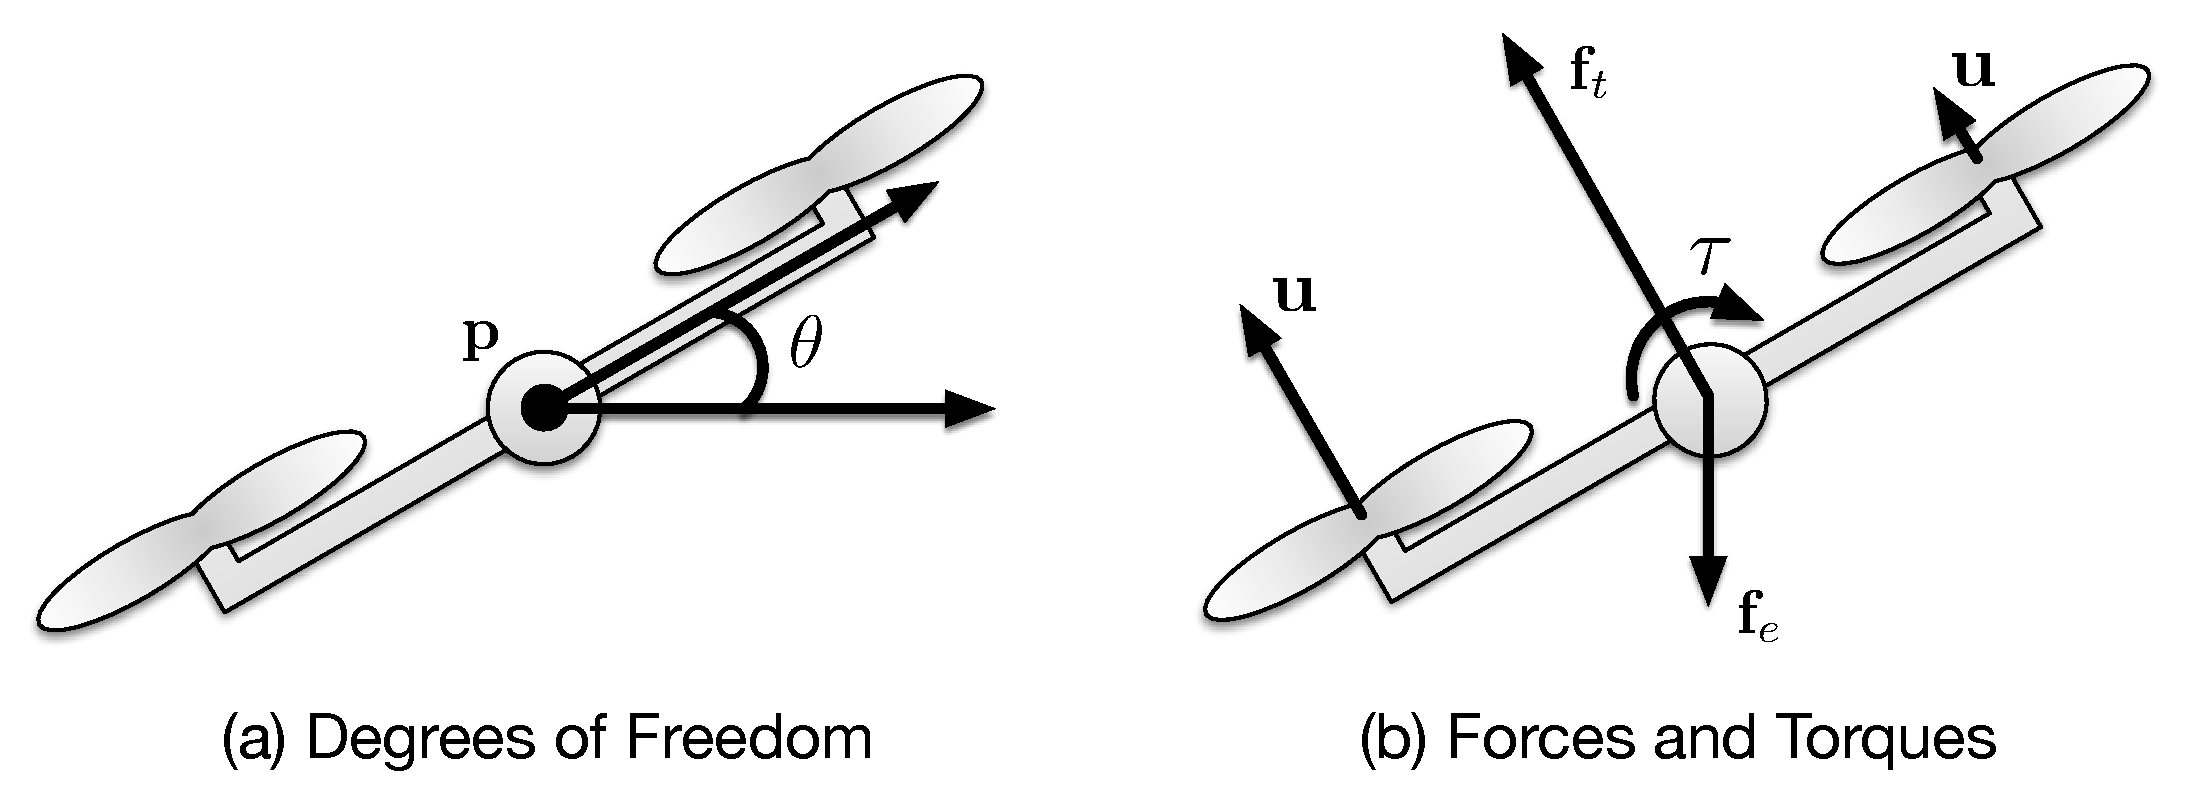
\includegraphics[width=4.0in]{images/2016_siggraph/10_model.pdf}
\caption{
Overview of our quadrotor dynamics model, shown in 2D for simplicity.
(a) Degrees of freedom. We model a quadrotor as having a position $\mathbf{p}$ and an orientation $\theta$.
(b) Forces and torques. We maneuver the quadrotor by applying a thrust force at each propellor, denoted with the vector $\mathbf{u}$.
These thrust forces generate a net thrust force $\mathbf{f}_t$ and a net torque $\mathbf{\tau}$ at the quadrotor's center of mass.
The only other force acting on the quadrotor is an external force $\mathbf{f}_e$, which models effects like gravity, wind, and drag.
This model does not include a camera gimbal, and is therefore lower-dimensional than the model in the previous chapter.
A lower-dimensional model is sufficient for our purposes in this chapter, because we guarantee that any drone with a two-axis gimbal can execute the camera trajectories produced by our algorithm.
}
\label{fig:ch3:model}
\end{figure}

In this section, we introduce the quadrotor dynamics model we use throughout this chapter.
Although this model is similar to the one in Chapter \ref{sec:ch2} and follows previous literature \cite{joubert:2015,mellinger:2011}, we present it here for completeness, and in a unified notation with the rest of the chapter.
We provide an overview of our model in Figure \ref{fig:ch3:model}.

\paragraph{Assumptions}

At a high level, we assume that we must maneuver a rigid body quadrotor equipped with a camera mounted on a gimbal. 
We assume that the quadrotor and gimbal are \emph{kinematically coupled} \cite{kondak:2013}, in the sense that moving the position of the quadrotor also moves the position of the gimbal.
However, we assume that our quadrotor and gimbal are not \emph{dynamically coupled} \cite{kondak:2013}, in the sense that torques acting on the gimbal do not induce reactive torques on the quadrotor.
We assume that the gimbal has very large actuator limits.

These assumptions simplify our dynamics model. 
In particular, our set of assumptions implies that, as long as we can maneuver the quadrotor to the correct position and heading, a 2-axis gimbal can always be oriented to match a desired camera pose.
This reasoning allows us to exclude the gimbal configuration and control torques from our dynamics model, resulting in a lower-dimensional and more computationally efficient model than the quadrotor camera model introduced in Chapter \ref{sec:ch2}.
We feel that these assumptions are reasonable, since the cameras mounted on quadrotors tend to be very lightweight relative to the quadrotors themselves.
For example, on our quadrotor hardware, the camera and gimbal are roughly 25$\times$ lighter than the actual quadrotor.

\paragraph{Degrees of Freedom, Control Forces, and Physical Limits}

We denote the degrees of freedom in our model with the vector $\mathbf{q}$.
This 6-dimensional vector contains the position and orientation of the quadrotor in the world frame.
We use Euler angles to represent the orientation of the quadrotor.
We refer to $\mathbf{q}$ as the \emph{configuration} of the quadrotor, and we refer to the space of all possible $\mathbf{q}$ values as the quadrotor's \emph{configuration space}. We denote the control forces in our model with the vector $\mathbf{u}$.
This 4-dimensional vector contains the magnitude of the upward thrust forces generated at each of the quadrotor's four propellers.
We refer to the space of all possible $\mathbf{u}$ values as the quadrotor's \emph{control space}.
We assume that our quadrotor can only achieve a limited speed in each dimension, and can only generate limited thrust at each propeller.
We express these limits as inequality constraints on $\dot{\mathbf{q}}$ and $\mathbf{u}$.
We relate the degrees of freedom in our  model to the control forces as follows,
%
\begin{equation}
\begin{aligned}
\mathbf{H}(\mathbf{q}) \ddot{\mathbf{q}} + \mathbf{C}(\mathbf{q},\dot{\mathbf{q}}) \dot{\mathbf{q}} + \mathbf{G}(\mathbf{q}) = \mathbf{B}(\mathbf{q}) \mathbf{u}\\
\text{subject to~~~~} \dot{\mathbf{q}}^{\text{min}} \leq \dot{\mathbf{q}} \leq \dot{\mathbf{q}}^{\text{max}}~~~~~~~~~\\
                      \mathbf{u}^{\text{min}}       \leq \mathbf{u}       \leq \mathbf{u}^{\text{max}}~~~~~~~~~\\
\end{aligned}
\label{eqn:ch3:manipulator}
\end{equation}
%
where
the matrix $\mathbf{H}$ models generalized inertia;
the matrix $\mathbf{C}$ models generalized velocity-dependent forces like drag;
the vector $\mathbf{G}$ models generalized potential forces like gravity;
the matrix $\mathbf{B}$ maps from control inputs to generalized forces;
and the inequalities represent the velocity limits and control force limits of our system.
These matrices can be obtained by expressing the quadrotor dynamics model presented by Mellinger and Kumar \shortcite{mellinger:2011} in matrix form (see Section \ref{sec:ch2:manipulator_detail} for a more detailed derivation).
In Section \ref{sec:ch3:manipulator}, we include a concise definition for these matrices, which are known as the \emph{manipulator matrices} \cite{tedrake:2016}.

\section{Solving for Velocities and Control Forces Along a Fixed Trajectory}
\label{sec:ch3:fixed_trajectory}

In this section, we use our model to solve in closed form for the velocities and control forces required to follow a user-specified camera trajectory.
As in Chapter \ref{sec:ch2}, we assume that the user's camera trajectory is $C^4$ continuous with respect to time.

Our approach in this section roughly follows the exposition in Chapter \ref{sec:ch2}.
However, we express our approach from a continuous perspective, rather than from a discrete perspective, since we rely on this continuous perspective to develop our analysis and optimization algorithm in Sections \ref{sec:ch3:fixed_path} and \ref{sec:ch3:optimization}.

At a high level, our approach is to solve for a trajectory through configuration space, that places the quadrotor at the same position and heading as the camera at all times.
We then substitute this \emph{configuration space trajectory} into equation (\ref{eqn:ch3:manipulator}) to solve for the corresponding \emph{control forces}.
Although the dynamics generally do not permit us to place the quadrotor at exactly the same orientation as the camera, we can always place it at the same heading.
As long as we place the quadrotor at the correct position with the correct heading, a 2-axis gimbal can always be oriented to achieve the desired camera pose.

\begin{Listing}[t]
\caption{
Computing the configuration of the quadrotor along a user-specified camera trajectory.
We begin by setting the quadrotor's position equal to the camera's position (line 1). We substitute linear acceleration and mass into Newton's Second Law to solve for net force (line 2).
We decompose the net force acting on our quadrotor into a thrust force and an external force, and we solve for thrust force (line 3).
We make the observation that a quadrotor can only generate thrust forces along its local up axis.
With this observation in mind, we set the quadrotor's local up axis equal to normalized thrust (line 4).
We use the quadrotor's local up axis, and the camera's look-at vector, to determine the quadrotor's orientation (lines 4--8).
This approach guarantees that the quadrotor's orientation is always consistent with equation (\ref{eqn:ch3:manipulator}).
%Or stated more precisely, that the configuration trajectories computed using this approach, when substituted into equation (\ref{eqn:manipulator}), always yield a left hand side that is in the column space of the matrix $\mathbf{B}$.
}
\label{lst:ch3:q}
\begin{algorithmic}[1]

\small

\REQUIRE { ~~\\ \vspace{-7pt}

\begin{itemize}
\item The current position, velocity, and acceleration of the camera in the world frame, $\mathbf{p}_c$, $\dot{\mathbf{p}}_c$, $\ddot{\mathbf{p}}_c$. \vspace{-7pt}
\item The camera's current look-at vector in the world frame, $\mathbf{x}_c$. \vspace{-7pt}
\item External force in the world frame, $\mathbf{f}_e$. \vspace{-7pt}
\item Mass of the quadrotor, $m$.
\end{itemize}

}

\ENSURE  { ~~\\ \vspace{-7pt}

\begin{itemize}
\item The quadrotor's current configuration, $\mathbf{q}$.
\end{itemize}

}

\STATE { $ \mathbf{p}_q                         \gets \mathbf{p}_c$ }
\STATE { $ \mathbf{f}                           \gets m\ddot{\mathbf{p}}_c$ }
\STATE { $ \mathbf{f}_t                         \gets \mathbf{f} - \mathbf{f}_e $ }
\STATE { $ \mathbf{y}_q                         \gets \text{normalized $\mathbf{f}_t$ } $ }
\STATE { $ \mathbf{z}_q                         \gets \text{normalized $\mathbf{y}_q \times \mathbf{x}_c$ } $ }
\STATE { $ \mathbf{x}_q                         \gets \text{normalized $\mathbf{z}_q \times \mathbf{y}_q$ } $ }
\STATE { $ \mathbf{R}_{\mathcal{Q},\mathcal{W}} \gets \text{the rotation matrix defined by the axes $\mathbf{x}_q$, $\mathbf{y}_q$, $\mathbf{z}_q$ } $ }
\STATE { $ \mathbf{e}_q                         \gets \text{the Euler angles corresponding to $\mathbf{R}_{\mathcal{Q},\mathcal{W}}$ } $ }
\STATE { $ \mathbf{q}                           \gets \begin{bmatrix} \mathbf{p}_q \\ \mathbf{e}_q \end{bmatrix} $ }

\end{algorithmic}
\end{Listing}

We provide an algorithm for computing the configuration of a quadrotor along a user-specified camera trajectory in Listing \ref{lst:ch3:q}.
This algorithm implicitly defines a closed form expression  for the quadrotor configuration $\mathbf{q}$ in terms of a user-specified camera trajectory.
We use the notation $\mathbf{Q}$ to refer to this closed form expression as follows,
%
\begin{equation}
\mathbf{q} = \mathbf{Q} (\mathbf{c},\dot{\mathbf{c}},\ddot{\mathbf{c}})
\label{eqn:ch3:q}
\end{equation}
%
where $\mathbf{c}$ is a stacked vector that includes the camera position $\mathbf{p}_c$ and the camera look-at vector $\mathbf{x}_c$.
The explicit form for $\mathbf{Q}$ can be obtained by proceeding sequentially through Listing \ref{lst:ch3:q}, symbolically substituting each line into the next.
However, the resulting expression for $\mathbf{Q}$ is quite verbose, so we omit it for brevity.

%Instead, we define the expression for $\mathbf{Q}$ implicitly according to the algorithm in Listing \ref{lst:q}. 

In order to solve for control forces, we need expressions for $\mathbf{q}$, $\dot{\mathbf{q}}$, and $\ddot{\mathbf{q}}$.
We obtain expressions for for $\dot{\mathbf{q}}$ and $\ddot{\mathbf{q}}$ by taking the derivative of equation (\ref{eqn:ch3:q}) twice with respect to time as follows,
%
\begin{equation}
\begin{aligned}
\dot{\mathbf{q}}  & = \frac{d \mathbf{Q}}{d t}     ~= \mathbf{\dot{\mathbf{Q}}}(\mathbf{c},\dot{\mathbf{c}},\ddot{\mathbf{c}},\dddot{\mathbf{c}} ) \\
\ddot{\mathbf{q}} & = \frac{d^2 \mathbf{Q}}{d t^2}  = \mathbf{\ddot{\mathbf{Q}}}(\mathbf{c},\dot{\mathbf{c}},\ddot{\mathbf{c}},\dddot{\mathbf{c}},\ddddot{\mathbf{c}} )
\end{aligned}
\label{eqn:ch3:qdotN}
\end{equation}
%
Finally, we solve for the control forces by substituting our expressions for $\mathbf{q}$, $\dot{\mathbf{q}}$, and $\ddot{\mathbf{q}}$ into equation (\ref{eqn:ch3:manipulator}) and solving for $\mathbf{u}$ as follows,
%
\begin{equation}
\mathbf{u} = \mathbf{B}^{\star}(\mathbf{q}) \left[\mathbf{H}(\mathbf{q}) \ddot{\mathbf{q}} + \mathbf{C}(\mathbf{q},\dot{\mathbf{q}}) \dot{\mathbf{q}} + \mathbf{G}(\mathbf{q})\right]
\label{eqn:ch3:u}
\end{equation}
%
where $\mathbf{B}^{\star}$ is the Moore-Penrose pseudoinverse of $\mathbf{B}$.
This approach is guaranteed to yield an exact unique solution for $\mathbf{u}$.
This is because we explicitly construct $\mathbf{q}$ to be consistent with the equations of motion for our system, so the left hand side of equation (\ref{eqn:ch3:manipulator}) is always in the column space of $\mathbf{B}$, and $\mathbf{B}$ is always full column rank \cite{joubert:2015}.
Since we have closed form expressions for $\mathbf{q}$, $\dot{\mathbf{q}}$, and $\ddot{\mathbf{q}}$, equation (\ref{eqn:ch3:u}) gives us a closed form expression for $\mathbf{u}$.
We use the notation $\mathbf{U}$ to refer to this closed form expression as follows,
%
\begin{equation}
\mathbf{u} = \mathbf{U}(\mathbf{c},\dot{\mathbf{c}},\ddot{\mathbf{c}},\dddot{\mathbf{c}},\ddddot{\mathbf{c}} )
\label{eqn:ch3:uc}
\end{equation}
%
Again, the explicit form for $\mathbf{U}$ is quite verbose, so we omit it for brevity.
At this point, we have solved in closed form for the velocities and control forces required to follow a user-specified camera trajectory.

\section{Solving for Velocities and Control Forces Along a Fixed Path with Variable Timing}
\label{sec:ch3:fixed_path}

In this section, we extend our analysis in Section \ref{sec:ch3:fixed_trajectory} to the case where only the camera \emph{path} is fixed by the user, but the camera's \emph{timing} can vary.
We begin by considering the camera's position and look-at vector as being parameterized by a scalar \emph{path parameter} $s \in [0,1]$.
We emphasize here that $s$ is not time; it is simply a parameter we can sweep from 0 to 1 to trace out our camera path.

In Section \ref{sec:ch3:fixed_trajectory}, we considered the camera position and look-at vector to be explicit functions of time.
In this section, we will instead consider these camera parameters to be explicit functions of our path parameter $s$, and we will consider our path parameter $s$ to be a function of time.
We express this \emph{implicit} dependence of our camera parameters on time as follows,
%
\begin{equation}
\mathbf{c} = \mathbf{c}(s(t))
\end{equation}
%
where $t$ is time.
We refer to the function $s(t)$ as the \emph{progress curve} along a path.
We assume that our camera parameters are $C^4$ continuous with respect to our path parameter $s$.

We factor the time derivatives of $\mathbf{c}$ using the chain rule as follows,
%
%\begin{equation}
%\dot{\mathbf{c}} = \frac{d \mathbf{c}}{d s} \frac{d s}{d t} = \mathbf{c}' \dot{s} \\
%\label{eqn:cdot}
%\end{equation}
%
%where we use the notation $\mathbf{c}'$ to refer to a derivative with respect to our path parameter $s$, and we use the notation $\dot{s}$ to refer to a derivative with respect to time.
%We can factor the higher derivatives of our camera parameters by repeatedly taking time derivatives of equation (\ref{eqn:cdot}) as follows,
%
\begin{equation}
\begin{aligned}
\dot{\mathbf{c}}    & = \mathbf{c}' \dot{s} \\
\ddot{\mathbf{c}}   & = \mathbf{c}''   \dot{s}^2 +   \mathbf{c}'   \ddot{s} \\
\dddot{\mathbf{c}}  & = \mathbf{c}'''  \dot{s}^3 + 3 \mathbf{c}''  \dot{s}   ~\ddot{s} +   \mathbf{c}'  \dddot{s} \\
\ddddot{\mathbf{c}} & = \mathbf{c}'''' \dot{s}^4 + 6 \mathbf{c}''' \dot{s}^2 ~\ddot{s} + 3 \mathbf{c}'' \ddot{s}^2 + 4 \mathbf{c}'' \dot{s}~\dddot{s} + \mathbf{c}' \ddddot{s}
\end{aligned}
\label{eqn:ch3:cdotn}
\end{equation}
%
where we use the notation $\mathbf{c}' = \frac{d \mathbf{c}}{d s}$ to indicate a derivative with respect to our path parameter $s$, and we use the notation $\dot{s} = \frac{d s}{d t}$ to indicate a derivative with respect to time.

We observe, remarkably, that velocities and control forces are fully determined by the progress curve along a fixed path.
To see that this is the case, we substitute equation (\ref{eqn:ch3:cdotn}) into our expressions for $\mathbf{q}$, $\dot{\mathbf{q}}$, $\ddot{\mathbf{q}}$, and $\mathbf{u}$ (i.e., into equations (\ref{eqn:ch3:q}), (\ref{eqn:ch3:qdotN}), and (\ref{eqn:ch3:uc})).
We find that we can express the full state of the quadrotor, and all necessary control forces, in terms of the functions  $\dot{s}(t)$, $\ddot{s}(t)$, $\dddot{s}(t)$, $\ddddot{s}(t)$, which can vary, and the functions $\mathbf{c}(s)$, $\mathbf{c}'(s)$, $\mathbf{c}''(s)$, $\mathbf{c}'''(s)$, $\mathbf{c}''''(s)$, which are fully determined by the fixed path.

We also observe that a progress curve must be $C^4$ continuous with respect to time in order for it to satisfy the quadrotor dynamics in equation (\ref{eqn:ch3:manipulator}).
This is because our expression for $\mathbf{u}$ depends on $\ddddot{\mathbf{c}}$, and $\ddddot{\mathbf{c}}$ depends on $\ddddot{s}$.

Together, these observations motivate the design of our optimization algorithm, described in Section \ref{sec:ch3:optimization}.



\section{Progress Curve Optimization}
\label{sec:ch3:optimization}

\begin{figure}[t]
\centering
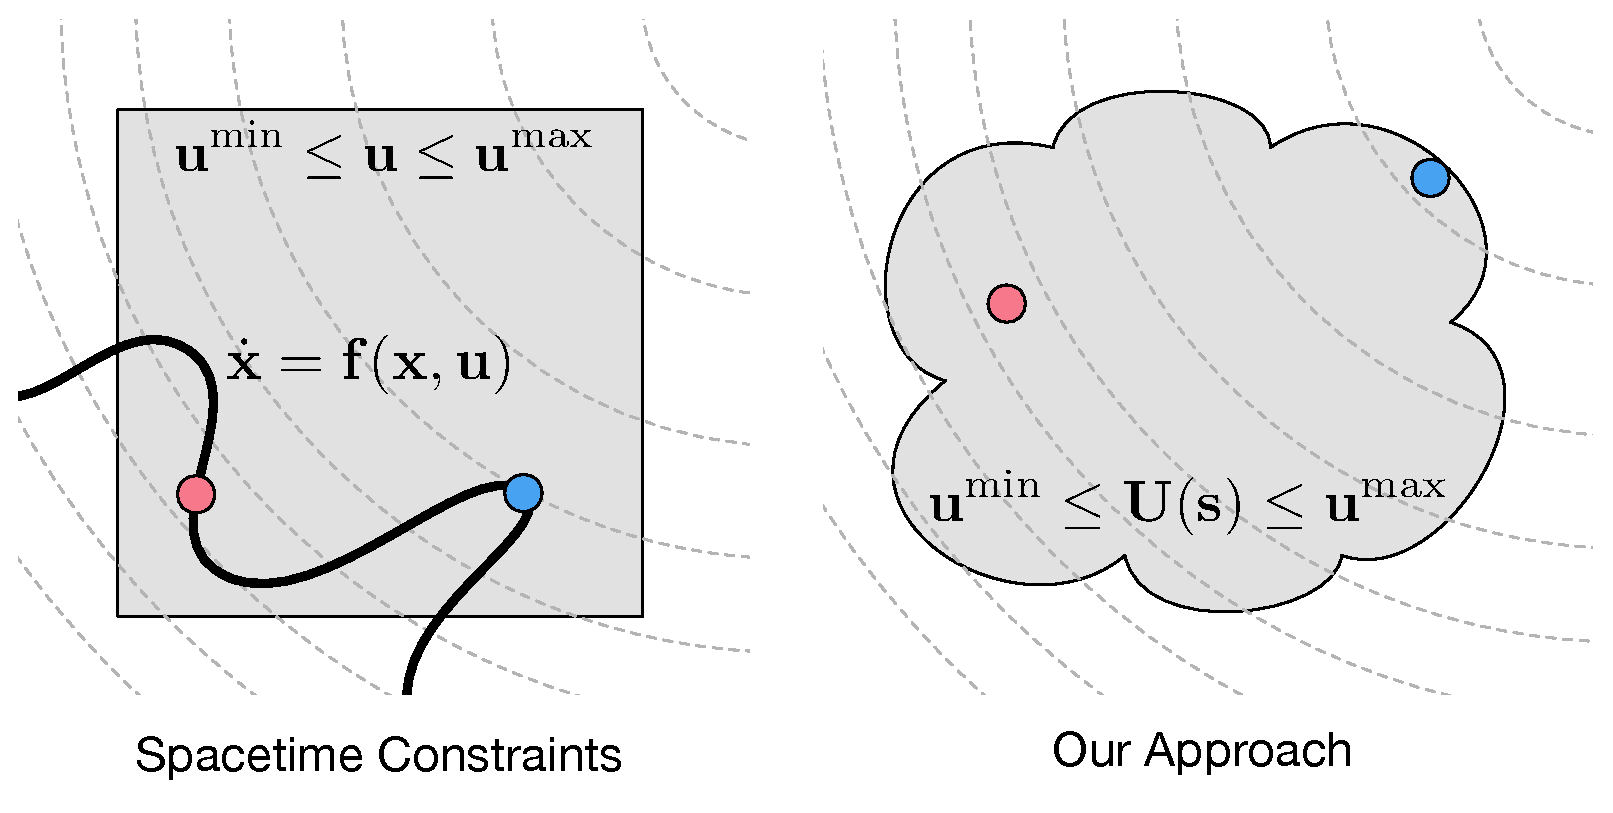
\includegraphics[width=4.0in]{images/2016_siggraph/22_optimization_problem_diagram.pdf}
\caption{
Illustration of the main difference between spacetime constraints (left) and our approach (right).
In spacetime con- straints, control force limits are easy to enforce, because they can be encoded as linear inequality constraints (grey shaded region, left).
However, quadrotor dynamics are hard to enforce, because they must be encoded as highly non-linear equality constraints (bold curve, left).
These non-linear equality constraints force a solver to take many small steps to get from an initial guess (red dot, left) to the optimal solution (blue dot, left).
In our approach, control force limits are more challenging to enforce, because they must be encoded as non-linear inequality constraints (grey shaded region, right).
However, our approach enforces the quadrotor dynamics implicitly, without requiring additional equality constraints.
Our approach enables a solver to make very rapid progress from an initial guess (red dot, right) to the optimal solution (blue dot, right).
}
\label{fig:ch3:optimization_problem_diagram}
\end{figure}

In Section \ref{sec:ch3:fixed_path}, we observed that the velocities and control forces required to fly a quadrotor along a fixed path, are fully determined by a progress curve along the path.
In this section, we optimize a progress curve to match a user-specified input progress curve as closely as possible, subject to velocity and control force limits.
We illustrate the main difference between spacetime constraints and our approach in Figure \ref{fig:ch3:optimization_problem_diagram}.

At a high level, we assume that we are given as input a user-specified camera path and progress curve. We discretize the camera path into a sequence of sample points, and we treat these sample points as fixed.
At each sample point, we solve for the progress curve \emph{time derivatives} that best agree with the user's input progress curve.
During this optimization procedure, we explicitly enforce $C^4$ continuity of our progress curve, as well as velocity and control force limits.
%We use the optimized speed profile to re-time the output trajectory, and compute a re-timed output trajectory
%After having solved for the optimal speed profile, we can easily recover a re-timing function, which we use to re-time the input trajectory.
In a simple post-processing step, we recover our output progress curve from the time derivatives.
After this post-processing step,  our output progress curve can be safely flown on a real quadrotor.

%\paragraph{Discretization}

%We begin by discretizing the user's camera path into $K$ samples.
%These samples do not need to be equally spaced.
%We also discretize the speed profile being optimized into $K$ samples, corresponding to discrete samples along the camera path.

\paragraph{Enforcing $C^4$ Continuity}

In our discrete problem, we must take care to enforce $C^4$ continuity of our progress curve with respect to time.
%For example, $\ddot{s}$ represents  the instantaneous change in $\dot{s}$.
%So, in our discrete problem, the change in our samples of $\dot{s}$ along the path should agree with the corresponding samples of $\ddot{s}$.
Stating this continuity constraint formally, let $\mathbf{s}_i$ be the first 4 time derivatives of our progress curve at sample point $i$.
Let $v_i$ be the \nth{5} time derivative of our progress curve at sample point $i$.
Let $dt_i$ be the time delta between sample points $i$ and $i+1$.
We enforce $C^4$ continuity of our progress curve as follows,
%
\begin{equation*}
\mathbf{s}_{i+1} = \mathbf{s}_{i} + (\mathbf{M}\mathbf{s}_{i} + \mathbf{N}v_{i})dt_i
\end{equation*}
%
\begin{equation}
\begin{aligned}
\text{subject to~~~~} & v^{\text{min}} \leq v_i \leq v^{\text{max}}\\
\text{where~~~~}      &
\mathbf{M} =
\begin{bmatrix}
0 & 1 & 0 & 0 \\
0 & 0 & 1 & 0 \\
0 & 0 & 0 & 1 \\
0 & 0 & 0 & 0
\end{bmatrix}
~~~~
\mathbf{N} =
\begin{bmatrix}
0 \\
0 \\
0 \\
1
\end{bmatrix}
\label{eqn:ch3:sip1}
\end{aligned}
\end{equation}
%
Mathematically speaking, this constraint does correctly enforce $C^4$ continuity.
However, since we intend to \emph{indirectly} optimize our progress curve by optimizing its time derivatives, we do not expect to have explicit access at optimization time to $dt_i$.
Therefore, we substitute $dt_i = \frac{ds_i}{\dot{s}_i}$ into equation (\ref{eqn:ch3:sip1}) to arrive at the following equality constraint,
%
\begin{equation}
\begin{aligned}
\mathbf{s}_{i+1} = \mathbf{s}_{i} + (\mathbf{M}\mathbf{s}_{i} + \mathbf{N}v_{i}) \frac{ds_i}{\dot{s}_i}
\end{aligned}
\end{equation}
%
In equation (\ref{eqn:ch3:sip1}), $v^{\text{min}}$ and $v^{\text{max}}$ control the extent to which $\ddddot{s}$ is allowed to vary from one sample point to the next, while still considering our progress curve to be $C^4$ continuous.
In our implementation, we set $v^{\text{min}}$ and $v^{\text{max}}$ heuristically, based on the minimum and maximum derivatives we observe in the input progress curve.
See Section \ref{sec:ch3:v_min_v_max} for details.

\paragraph{Enforcing Forward Progress}
In our discrete problem, we must take care to ensure that the quadrotor always makes forward progress along the path.
Or stated more precisely, we must enforce the constraint that $\dot{s} > 0$.
Again, since we indirectly optimize our progress curve by optimizing its time derivatives, this constraint ensures that our optimized progress curve always reaches the end of the path.

\paragraph{Full Optimization Problem}
Stating our optimization problem formally, let $\mathbf{S}$ be the concatenated vector of all $\mathbf{s}_i$ values along the path.
Similarly, let $\mathbf{V}$ be the concatenated vector of all $v_i$ values along the path.
Let $\dot{s}_i^{\text{ref}}$ be the \nth{1} time derivative of the user's input progress curve at sample point $i$.
We would like to find the the optimal set of progress curve time derivatives $\mathbf{S}^*$ and $\mathbf{V}^*$ as follows, 
%
\begin{equation*}
\begin{aligned}
\mathbf{S}^{*},\mathbf{V}^{*} & = \argmin_{\mathbf{S},\mathbf{V}} \sum_{i} ( \dot{s}_i - \dot{s}_i^{\text{ref}} )^{2} \\
\text{subject to~~~~}
\mathbf{s}_{i+1}              & =    \mathbf{s}_{i} + (\mathbf{M}\mathbf{s}_{i} + \mathbf{N}v_{i}) \frac{ds_i}{\dot{s}_i} \\
\end{aligned}
\end{equation*}
%
\vspace{-5pt}
\begin{equation}
\begin{aligned}
v^{\text{min}}  & \leq v_i \leq v^{\text{max}} & \dot{\mathbf{q}}^{\text{min}}  \leq \dot{\mathbf{Q}}(\mathbf{s}_i) \leq \dot{\mathbf{q}}^{\text{max}} \\
\dot{s}_i       & > 0                          & \mathbf{u}^{\text{min}}          \leq \mathbf{U}(\mathbf{s}_i)       \leq \mathbf{u}^{\text{max}} \\
\end{aligned}
\label{eqn:ch3:s_star_v_star}
\end{equation}
%
The objective function in this optimization problem attempts to match the optimized progress curve with the input progress curve as closely as possible.
The equality constraints, and the inequality constraints on $v_i$, enforce $C^4$ continuity of the progress curve.
The inequality constraint on $\dot{s}_i$ ensures that the progress curve always reaches the end of the path.
The other inequality constraints enforce velocity and control force limits.
We use the notation $\dot{\mathbf{Q}}(\mathbf{s}_i)$ and $\mathbf{U}(\mathbf{s}_i)$ to refer to our closed form expressions for velocities and control forces, expressed entirely in terms of our progress curve time derivatives, as described in Section \ref{sec:ch3:fixed_path}.
$\mathbf{S}$ and $\mathbf{V}$ are decision variables, everything else is problem data.

%The objective function in our optimization problem is quadratic, but the contraints are non-convex.
%Therefore, we solve our problem in (\ref{eqn:s_star_v_star}) using the commercially available non-convex solver SNOPT.

\paragraph{Improving Computational Efficiency}

\begin{figure*}[t]
\centering
\includegraphics[width=6.0in]{images/2016_siggraph/21_real_footage.pdf}
\caption{
Side-by-side comparison of a \textsc{Google Earth} shot preview (top row) and real video footage (bottom row) from an aggressive trajectory generated using our algorithm.
Our algorithm produces trajectories that can be faithfully captured on a real quadrotor, even when the trajectories are at the quadrotor's physical limits.
}
\label{fig:ch3:real}
\end{figure*}

To improve computational efficiency, we make two important approximations to the problem in (\ref{eqn:ch3:s_star_v_star}).

%First, we can drastically improve performance by providing a non-convex solver with callback functions to compute the analytic derivatives of our objective function, and our constraint functions, with respect to our decision variables.
%These analytic derivatives can be very time-consuming and error prone to derive manually, and therefore we use the symbolic algebra library SymPy [CITE] to compute them automatically. 
%However, we found that computing an analytic expression for $\frac{ \partial \mathbf{U} }{ \partial \mathbf{s}_i } $ was not possible in a reasonable amount of time due to the factorial (in the number of mathematical symbols) complexity of the pseudoinverse term  in equation (\ref{eqn:u}).
%Moreover, even if we did successfully pre-compute an analytic expression for $\frac{ \partial \mathbf{U} }{ \partial \mathbf{s}_i } $, it would be expensive to evaluate at optimization time.

First, in order for our non-convex solver to achieve acceptable performance, we must compute analytic derivatives of our objective function, and our constraint functions, with respect to our decision variables.
We use the symbolic algebra library SymPy to compute these analytic derivatives \cite{sympy:2014}.
However, we found that computing an analytic expression for $\frac{ \partial \mathbf{U} }{ \partial \mathbf{s}_i } $ was not possible in a reasonable amount of time due to the factorial (in the number of mathematical symbols) complexity of the pseudoinverse term  in equation (\ref{eqn:ch3:u}).
Therefore, we use the following approximation for equation (\ref{eqn:ch3:u}),
%
\begin{equation}
\bar{\mathbf{u}} = \bar{\mathbf{B}}^{\star} \left[\mathbf{H}(\mathbf{q}) \ddot{\mathbf{q}} + \mathbf{C}(\mathbf{q},\dot{\mathbf{q}}) \dot{\mathbf{q}} + \mathbf{G}(\mathbf{q})\right]
\label{eqn:ch3:uhat}
\end{equation}
%
where $\bar{\mathbf{B}}^{\star}$ is a constant (for the purpose of computing analytic derivatives) approximation of $\mathbf{B}^{\star}(\mathbf{q})$.

%We note that our previous analysis in Sections \ref{sec:fixed_trajectory} and \ref{sec:fixed_path} also applies to $\hat{\mathbf{u}}$, in the sense that we can express  $\hat{\mathbf{u}}$ completely in terms of our speed profile decision variables.
%Our second approximation is similar to our first, and is motivated by the observation that the equality constraints in problem (\ref{eqn:s_star_v_star}) are \emph{nearly} linear.

Second, we would prefer for our equality constraints to be linear, since this would make more of our problem convex, and therefore more computationally efficient \cite{boyd:2008}.
With this reasoning in mind, we replace our \emph{nearly} linear equality constraints with the following linear approximations,
%
\begin{equation}
\mathbf{s}_{i+1} = \mathbf{s}_{i} + (\mathbf{M}\mathbf{s}_{i} + \mathbf{N}\mathbf{v}_{i}) \frac{ds_i}{\bar{\dot{s}}_i}
\end{equation}
%
where $\bar{\dot{s}}_i$ is a constant (for the purpose of computing analytic derivatives) approximation of $\dot{s}_i$.
%After having made this approximation, the equality constraints in our problem become linear.

Although we treat $\bar{\mathbf{B}}^{\star}$ and $\bar{\dot{s}}$ as constant for the purpose of computing analytic derivatives, we iteratively refine the values of $\bar{\mathbf{B}}^{\star}$ and $\bar{\dot{s}}$ as our solver makes progress towards a solution, according to the following update rules,
%To perform these refinements, we use values available from the solver's previous iteration, according to the following update rules,
%
\begin{equation}
\bar{\mathbf{B}}^{\star [i]} = \mathbf{B}^{\star}(\mathbf{q}^{[i-1]}) ~~~~~~~~~~~~ \bar{\dot{s}}^{[i]} = \dot{s}^{[i-1]}
\end{equation}
%
where the superscript notation refers to our solver's iteration count.
Boyd refers to this strategy as \emph{quasi-linearization} \shortcite{boyd:2008}.

To further improve the convergence behavior of our algorithm, at the expense of a modest reduction in accuracy, we simply stop updating $\bar{\dot{s}}$ after a small fixed number of iterations.
In all the results shown in this chapter, we stop updating $\bar{\dot{s}}$ after 10 iterations.
We evaluate the speed and accuracy tradeoffs associated with this choice in Section \ref{sec:ch3:results}.

\paragraph{Fast Approximate Optimization Problem}

Based on the approximations described in the previous subsection, we express our fast approximate optimization problem as follows, 
%
\begin{equation*}
\begin{aligned}
\mathbf{S}^{*},\mathbf{V}^{*} & = \argmin_{\mathbf{S},\mathbf{V}} \sum_{i} ( \dot{s}_i - \dot{s}_i^{\text{ref}} )^{2} \\
\text{subject to~~~~}
\mathbf{s}_{i+1}              & =    \mathbf{s}_{i} + (\mathbf{M}\mathbf{s}_{i} + \mathbf{N}v_{i}) \frac{ds_i}{\bar{\dot{s}}_i} \\
\end{aligned}
\end{equation*}
%
\begin{equation}
\begin{aligned}
v^{\text{min}}  & \leq v_i \leq v^{\text{max}} & \dot{\mathbf{q}}^{\text{min}} \leq \dot{\mathbf{Q}}(\mathbf{s}_i) \leq \dot{\mathbf{q}}^{\text{max}} \\
\dot{s}_i       & > 0                                   & \mathbf{u}^{\text{min}}       \leq \bar{\mathbf{U}}(\mathbf{s}_i)       \leq \mathbf{u}^{\text{max}} \\
\end{aligned}
\label{eqn:ch3:s_star_v_star_approx}
\end{equation}
%
where $\bar{\mathbf{U}}(\mathbf{s}_i)$ is our closed form expression for control forces that includes the approximation from equation (\ref{eqn:ch3:uhat}).
The problem in (\ref{eqn:ch3:s_star_v_star_approx}) is expressed in a standard form that can be given directly to an off-the-shelf solver.
In our implementation, we solve the problem in (\ref{eqn:ch3:s_star_v_star_approx}) using the commercially available non-convex solver SNOPT \cite{gill:2002}.

%Once we have a solution to the problem in (\ref{eqn:s_star_v_star_approx}), we can easily obtain the re-timing function that maps input times to output times.
%To compute this re-timing function, we simply compute the time deltas between sample points according to $dt_i = \frac{ds_i}{\dot{s}_i}$.
%Finally, we cumulatively sum the time deltas to obtain a sequence of output times.

\paragraph{Initialization}

The optimization problem in (\ref{eqn:ch3:s_star_v_star_approx}) is non-convex, and is therefore sensitive to initialization.
We initialize our solver by uniformly time stretching the input progress curve until it becomes feasible.
Next, we compute the time derivatives of the uniformly stretched progress curve, and we use these time derivatives to initialize our solver.
When computing these time derivatives, we take care to compute numerical derivatives using the same forward differencing scheme as in equation (\ref{eqn:ch3:sip1}).
In our experience, this initialization strategy noticeably improves the convergence behavior of our solver, compared to initializing with the original infeasible input progress curve.
We speculate that this improvement occurs because our constraint gradients are relatively well-behaved near hover conditions, but become increasingly oscillatory and non-convex far away from hover conditions.
Therefore, initializing with an overly conservative feasible trajectory, rather than an overly aggressive infeasible trajectory, allows our solver to take advantage of more globally meaningful gradient information.

